\label{ap:ap09}
\chapter{Deep learning}
\section*{\textbf{A - ENUNCIADO}}

\subsection*{\textbf{1 Classificação de Imagens (CNN)}}



Implementar o exemplo de classificação de objetos usando a base de dados CIFAR10 e a arquitetura CNN vista no curso.



\subsection*{\textbf{2 Detector de SPAM (RNN)}}



\textcolor{black}{Implementar o detector de spam visto em sala, usando a base de dados SMS Spam e arquitetura de RNN
vista no curso.}



\subsection*{\textbf{3 Gerador de Dígitos Fake (GAN)}}



\textcolor{black}{Implementar o gerador de dígitos }\textit{\textcolor{black}{fake}}\textcolor{black}{ usando a base de
dados MNIST e arquitetura GAN vista no curso.}



\subsection*{\textbf{4 Tradutor de Textos (Transformer)}}



\textcolor{black}{Implementar o tradutor de texto do português para o inglês, usando a base de dados e a arquitetura
Transformer vista no curso.}

%%%%%%%%%%%%%%%%%%%%%%%%%%%%%%%%%%%%%%%%%%%%%%%%%%%%%%%%%%%%%%%%%%%%%%%%%%%%%%%%%%%%%%%%%%%%%
\section*{\textbf{B - RESOLUÇÃO}}
\begin{adjustwidth}{1em}{}
\textbf{1 Classificação de Imagens (CNN)}
\end{adjustwidth}

\begin{lstlisting}[language=Python, style=input]
import tensorflow as tf
import numpy as np
import matplotlib.pyplot as plt
from tensorflow.keras.layers import Input, Conv2D, Dense, Flatten, Dropout
from tensorflow.keras.models import Model
from mlxtend.plotting import plot_confusion_matrix
from sklearn.metrics import confusion_matrix

# Carga da base
cifar10 = tf.keras.datasets.cifar10
# Já está separado em dados de treino e teste
# Não precisa separar
(x_train, y_train), (x_test, y_test) = cifar10.load_data()

# Normalização os dados
# Imagens em pixels de 0 - 255
# / 255.0 transforma em 0 - 1
x_train, x_test = x_train / 255.0, x_test / 255.0
# O dado y é a classe a qual faz parte
# O flattem torna os dados vetorizados
y_train, y_test = y_train.flatten(), y_test.flatten()

K = len(set(y_train))
# Aqui começa o Estágio 1
i = Input(shape=x_train[0].shape)
x = Conv2D(32, (3, 3), strides=2, activation="relu")(i)
x = Conv2D(64, (3, 3), strides=2, activation="relu")(x)
x = Conv2D(128, (3, 3), strides=2, activation="relu")(x)
# Todas as imagens são do mesmo tamanho, não precisa de Global Pooling
x = Flatten()(x)
# Aqui começa o Estágio 2
x = Dropout(0.5)(x)
x = Dense(1024, activation="relu")(x)
x = Dropout(0.2)(x)
x = Dense(K, activation="softmax")(x)
# Model ( lista entrada, lista saída)
model = Model(i, x)

model.summary()
\end{lstlisting}

\begin{tcolorbox}[myoutputstyle]
Model: "functional"\\

\begin{tabular}{|l|l|r|}
\hline
\textbf{Layer (type)} & \textbf{Output Shape} & \textbf{Param \#} \\ \hline
input\_layer (InputLayer) & (None, 32, 32, 3) & 0 \\ \hline
conv2d (Conv2D) & (None, 15, 15, 32) & 896 \\ \hline
conv2d\_1 (Conv2D) & (None, 7, 7, 64) & 18,496 \\ \hline
conv2d\_2 (Conv2D) & (None, 3, 3, 128) & 73,856 \\ \hline
flatten (Flatten) & (None, 1152) & 0 \\ \hline
dropout (Dropout) & (None, 1152) & 0 \\ \hline
dense (Dense) & (None, 1024) & 1,180,672 \\ \hline
dropout\_1 (Dropout) & (None, 1024) & 0 \\ \hline
dense\_1 (Dense) & (None, 10) & 10,250 \\ \hline
\end{tabular}\\

Total params: 1,284,170 (4.90 MB)\\
Trainable params: 1,284,170 (4.90 MB)\\
Non-trainable params: 0 (0.00 B)\\
\end{tcolorbox}


\begin{lstlisting}[language=Python, style=input]
# Compilar o modelo
model.compile(optimizer="adam",
loss="sparse_categorical_crossentropy", metrics=["accuracy"])
# Treinar o modelo
r = model.fit(x_train, y_train, validation_data=(x_test, y_test),
epochs=15)

# Plotar a função de perda, treino e validação
plt.plot(r.history["loss"], label="loss")
plt.plot(r.history["val_loss"], label="val_loss")
plt.legend()
plt.show()

# Plotar acurácia, treino e validação
plt.plot(r.history["accuracy"], label="acc")
plt.plot(r.history["val_accuracy"], label="val_acc")
plt.legend()
plt.show()
\end{lstlisting}

\begin{figure}[H]
\centering
\caption{Função de perda - CNN}
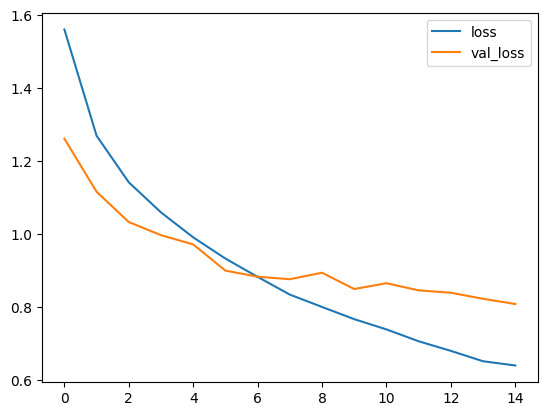
\includegraphics[width=.8\linewidth]{apendices/fig/9_IAA009_1.png}
\caption*{Fonte: O autor (2024).}
\end{figure}

\begin{figure}[H]
\centering
\caption{Acurácia - CNN}
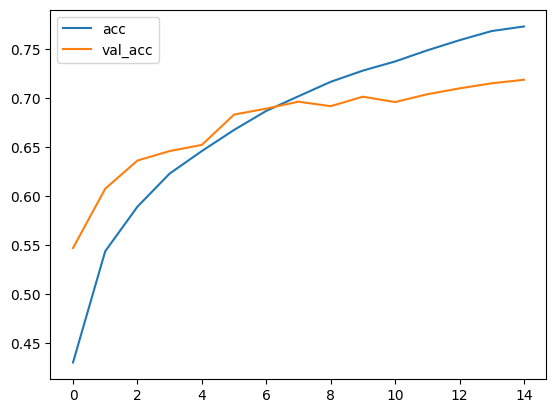
\includegraphics[width=.8\linewidth]{apendices/fig/9_IAA009_2.png}
\caption*{Fonte: O autor (2024).}
\end{figure}


\begin{lstlisting}[language=Python, style=input]
# Efetuar predições na base de teste
# argmax é usado pois a função de ativação da saída é softmax
# argmax pega o neurônio que deu o maior resultado, isto é,
# a maior probabilidade de saída
y_pred = model.predict(x_test).argmax(axis=1)
# Mostrar a matriz de confusão
cm = confusion_matrix(y_test, y_pred)
plot_confusion_matrix(conf_mat=cm, figsize=(7, 7),
show_normed=True)
\end{lstlisting}

\begin{figure}[H]
\centering
\caption{Matriz de confusão - CNN}
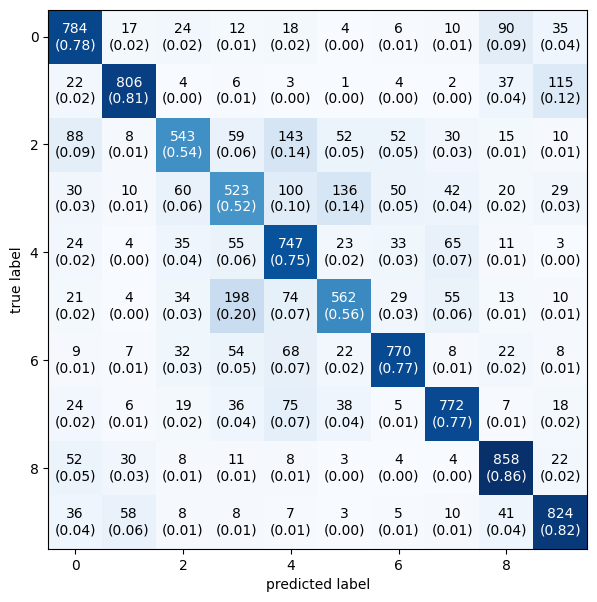
\includegraphics[width=.8\linewidth]{apendices/fig/9_IAA009_3.png}
\caption*{Fonte: O autor (2024).}
\end{figure}

\begin{lstlisting}[language=Python, style=input]
# Mostrar algumas classificações erradas
labels= ["airplane", "automobile", "bird", "cat", "deer", "dog",
"frog", "horse", "ship", "truck"]
misclassified = np.where(y_pred != y_test)[0]
i = np.random.choice(misclassified)
plt.imshow(x_test[i], cmap="gray")
plt.title("True label: %s Predicted: %s" % (labels[y_test[i]],
labels[y_pred[i]]))
\end{lstlisting}

\begin{figure}[H]
\centering
\caption{Classificação errada - CNN}
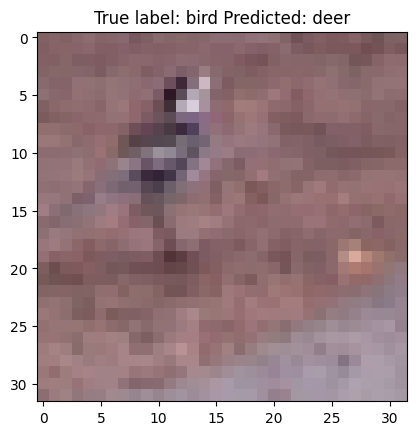
\includegraphics[width=.8\linewidth]{apendices/fig/9_IAA009_4.png}
\caption*{Fonte: O autor (2024).}
\end{figure}

\begin{adjustwidth}{1em}{}
\textbf{2 Detector de SPAM (RNN)}
\end{adjustwidth}
\begin{lstlisting}[language=Python, style=input]
# Importação das Bibliotecas
import tensorflow as tf
import numpy as np
import matplotlib.pyplot as plt
import pandas as pd
from sklearn.model_selection import train_test_split
from tensorflow.keras.layers import Input, Embedding, LSTM, Dense
from tensorflow.keras.layers import GlobalMaxPooling1D
from tensorflow.keras.models import Model
from tensorflow.keras.preprocessing.sequence import pad_sequences
from tensorflow.keras.preprocessing.text import Tokenizer

# carrega e arruma a base
!wget http://www.razer.net.br/datasets/spam.csv
# !wget https://www.kaggle.com/datasets/uciml/sms-spam-collection-dataset
df = pd.read_csv("spam.csv", encoding="ISO-8859-1")
df.head()
df = df.drop(["Unnamed: 2", "Unnamed: 3", "Unnamed: 4"], axis=1)
df.columns = ["labels", "data"]
df["b_labels"] = df["labels"].map({ "ham": 0, "spam": 1})
y = df["b_labels"].values

# Separa a base em treino e teste
x_train, x_test, y_train, y_test = train_test_split(df["data"], y,
test_size=0.33)

# Número máximo de palavras para considerar
# São consideradas as mais frequentes, as demais são
#   ignoradas
num_words = 20000
tokenizer = Tokenizer(num_words=num_words)
tokenizer.fit_on_texts(x_train)
sequences_train = tokenizer.texts_to_sequences(x_train)
sequences_test = tokenizer.texts_to_sequences(x_test)
word2index = tokenizer.word_index
V = len(word2index)

# Acerta o tamanho das sequências (padding)
data_train = pad_sequences(sequences_train) # usa o tamanho da maior seq.
T = data_train.shape[1] # tamanho da sequência
data_test = pad_sequences(sequences_test, maxlen=T)
print("%s tokens" % V)
print("data_train.shape: ", data_train.shape)
print("data_test.shape: ", data_test.shape)
\end{lstlisting}

\begin{tcolorbox}[myoutputstyle]
7201 tokens\\
data\_train.shape:  (3733, 189)\\
data\_test.shape:  (1839, 189)
\end{tcolorbox}


\begin{lstlisting}[language=Python, style=input]
# Define o modelo
D = 20   # tamanho do embedding, hiperparâmetro que pode ser escolhido
M = 5    # tamanho do hidden state, quantidade de unidades LSTM
i = Input(shape=(T,)) # Entra uma frase inteira
x = Embedding(V+1, D)(i)
x = LSTM(M)(x)
x = Dense(1, activation="sigmoid")(x) # Sigmoide pois só tem 2 valores
model = Model(i, x)
model.summary()
\end{lstlisting}

\begin{tcolorbox}[myoutputstyle]
Model: "functional"
\begin{table}[H]
%\centering
\begin{tabular}{|l|c|r|}
\hline
\textbf{Layer (type)} & \textbf{Output Shape} & \textbf{Param \#} \\ \hline
input\_layer (InputLayer) & (None, 189) & 0 \\ \hline
embedding (Embedding) & (None, 189, 20) & 143,980 \\ \hline
lstm (LSTM) & (None, 5) & 520 \\ \hline
dense (Dense) & (None, 1) & 6 \\ \hline
\end{tabular}
%\caption{Model summary}
\end{table}
 Total params: 144,506 (564.48 KB)\\
 Trainable params: 144,506 (564.48 KB)\\
 Non-trainable params: 0 (0.00 B)
\end{tcolorbox}

\begin{lstlisting}[language=Python, style=input]
# Compila e treina o modelo
model.compile(loss="binary_crossentropy", optimizer="adam",
metrics=["accuracy"])
epochs = 5
r = model.fit(data_train, y_train, epochs=epochs, validation_data=(data_test,
y_test))

# Plota função de perda e acurácia
plt.plot(r.history["loss"], label="loss")
plt.plot(r.history["val_loss"], label="val_loss")
plt.xlabel("Epocas")
plt.ylabel("loss")
plt.xticks(np.arange(0, epochs, step=1), labels=range(1, epochs+1))
plt.legend()
plt.show()
plt.plot(r.history["accuracy"], label="accuracy")
plt.plot(r.history["val_accuracy"], label="val_accuracy")
plt.xlabel("Epocas")
plt.ylabel("Acurácia")
plt.xticks(np.arange(0, epochs, step=1), labels=range(1, epochs+1))
plt.legend()
plt.show()
\end{lstlisting}


\begin{figure}[H]
\centering
\caption{Função de perda - RNN}
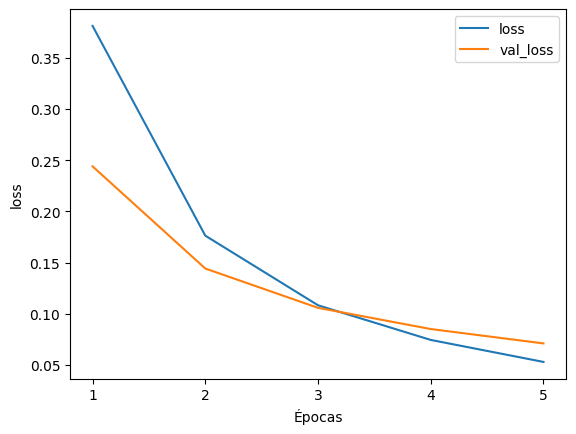
\includegraphics[width=.8\linewidth]{apendices/fig/9_IAA009_5.png}
\caption*{Fonte: O autor (2024).}
\end{figure}

\begin{figure}[H]
\centering
\caption{Acurácia - RNN}
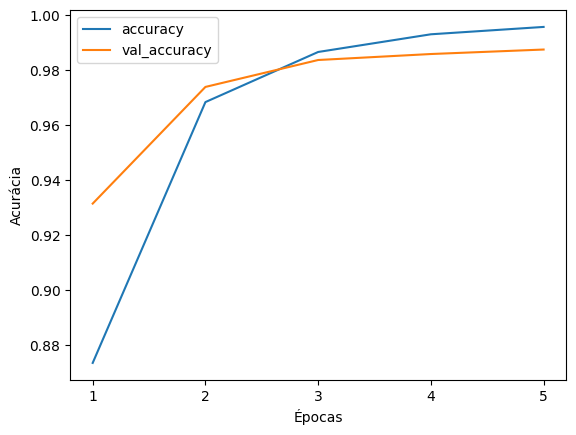
\includegraphics[width=.8\linewidth]{apendices/fig/9_IAA009_6.png}
\caption*{Fonte: O autor (2024).}
\end{figure}

\begin{lstlisting}[language=Python, style=input]
# Efetua a predição de um texto novo
#texto = "Hi, my name is Razer and want to tell you something."
texto = "Is your car dirty? Discover our new product. Free for all. Click the link."
seq_texto = tokenizer.texts_to_sequences([texto]) # Tokeniza
data_texto = pad_sequences(seq_texto, maxlen=T)   # Padding
pred = model.predict(data_texto) # Predição
print(pred)
print ("SPAM" if pred >= 0.5 else "OK")
\end{lstlisting}

\begin{tcolorbox}[myoutputstyle]
[[0.7768526]]\\
SPAM
\end{tcolorbox}


%%%%%%%%%%%%%%%%%%%%%%%%%%%%%%%%%%%%%%%%%%%%%%%%%%%%%%%%%%%%%%%%%%%%%%%%%%%%%%%%%%%%%%%%%%%
\begin{adjustwidth}{1em}{}
\textbf{3 Gerador de Dígitos Fake (GAN)}
\end{adjustwidth}

\begin{lstlisting}[language=Python, style=input]
!pip install imageio
!pip install git+https://github.com/tensorflow/docs

# Importações
import tensorflow as tf
import glob
import imageio
import matplotlib.pyplot as plt
import numpy as np
import os
import PIL
from tensorflow.keras import layers
import time
from IPython import display

# Carregar a base de dados
(train_images, train_labels), (_, _) = tf.keras.datasets.mnist.load_data()
# Normalização
train_images = train_images.reshape(train_images.shape[0], 28, 28, 1).astype('float32')
train_images = (train_images - 127.5) / 127.5  # Normaliza entre [-1, 1]
# Gera o banco em partes e randomiza
BUFFER_SIZE = 60000
BATCH_SIZE = 256
# Cria o dataset (from_tensor_slices)
# Randomiza (shuffle)
# Combina elementos consecutivos em lotes (batch)
train_dataset = tf.data.Dataset.from_tensor_slices(train_images).shuffle(BUFFER_SIZE).batch(BATCH_SIZE)

# Cria o GERADOR
def make_generator_model():
  model = tf.keras.Sequential()
  model.add(layers.Dense(7*7*256, use_bias=False,input_shape=(100,)))
  model.add(layers.BatchNormalization())
  model.add(layers.LeakyReLU())

  model.add(layers.Reshape((7, 7, 256)))
  assert model.output_shape == (None, 7, 7, 256)

  # Note: None is the batch size
  model.add(layers.Conv2DTranspose(128, (5, 5), strides=(1, 1), padding='same', use_bias=False))
  assert model.output_shape == (None, 7, 7, 128)

  model.add(layers.BatchNormalization())
  model.add(layers.LeakyReLU())

  model.add(layers.Conv2DTranspose(64, (5, 5), strides=(2, 2), padding='same', use_bias=False))
  assert model.output_shape == (None, 14, 14, 64)
  model.add(layers.BatchNormalization())
  model.add(layers.LeakyReLU())

  model.add(layers.Conv2DTranspose(1, (5, 5), strides=(2, 2), padding='same', use_bias=False, activation='tanh'))
  assert model.output_shape == (None, 28, 28, 1)
  return model

# Teste do GERADOR, ainda não treinado
generator = make_generator_model()

noise = tf.random.normal([1, 100])
generated_image = generator(noise, training=False)

plt.imshow(generated_image[0, :, :, 0], cmap='gray')
\end{lstlisting}

\begin{figure}[H]
\centering
\caption{Teste gerador - GAN}
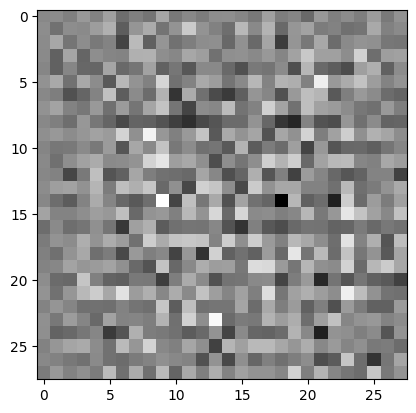
\includegraphics[width=.7\linewidth]{apendices/fig/9_IAA009_7.png}
\caption*{Fonte: O autor (2024).}
\end{figure}


\begin{lstlisting}[language=Python, style=input]
# Cria o DISCRIMINADOR
def make_discriminator_model():
  model = tf.keras.Sequential()
  model.add(layers.Conv2D(64, (5, 5), strides=(2, 2), padding='same', input_shape=[28, 28, 1]))
  model.add(layers.LeakyReLU())
  model.add(layers.Dropout(0.3))

  model.add(layers.Conv2D(128, (5, 5), strides=(2, 2), padding='same'))
  model.add(layers.LeakyReLU())
  model.add(layers.Dropout(0.3))

  model.add(layers.Flatten())
  model.add(layers.Dense(1))
  return model

# Teste do DISCRIMINADOR, ainda não treinado
discriminator = make_discriminator_model()
decision = discriminator(generated_image)
#print (decision)

# Define as funções de perda
cross_entropy = tf.keras.losses.BinaryCrossentropy(from_logits=True)

# Perda do DISCRIMINADOR
def discriminator_loss(real_output, fake_output):
  real_loss = cross_entropy(tf.ones_like(real_output), real_output)
  fake_loss = cross_entropy(tf.zeros_like(fake_output), fake_output)
  total_loss = real_loss + fake_loss
  return total_loss

# Perda do GERADOR
def generator_loss(fake_output):
  return cross_entropy(tf.ones_like(fake_output), fake_output)

# Cria os otimizadores para o gerador e discriminador
generator_optimizer = tf.keras.optimizers.Adam(1e-4)
discriminator_optimizer = tf.keras.optimizers.Adam(1e-4)

# Cria checkpoints para salvar modelos ao longo do tempo
# Uteis em tarefas longas, para se recuperar de um desligamento
checkpoint_dir = './training_checkpoints'
checkpoint_prefix = os.path.join(checkpoint_dir, "ckpt")
checkpoint = tf.train.Checkpoint(generator_optimizer=generator_optimizer,
                                 discriminator_optimizer=discriminator_optimizer,
                                 generator=generator,
                                 discriminator=discriminator)

                             # Configura o Loop de treinamento
EPOCHS = 100
noise_dim = 100
num_examples_to_generate = 16
# You will reuse this seed overtime (so it's easier)
# to visualize progress in the animated GIF)
seed = tf.random.normal([num_examples_to_generate, noise_dim])

def f(x, y):
  return 3*x**2 + 2*x*y

x, y = tf.Variable(5.), tf.Variable(3.)
with tf.GradientTape() as tape:
  z = f(x, y)
gradients = tape.gradient(z, [x, y])
print(gradients)

# Função que faz um passo de treinamento
# E uma tf.function, que compila essa funcao
@tf.function
def train_step(images):
  noise = tf.random.normal([BATCH_SIZE, noise_dim])

  with tf.GradientTape() as gen_tape, tf.GradientTape() as disc_tape:
    generated_images = generator(noise, training=True)

    real_output = discriminator(images, training=True)
    fake_output = discriminator(generated_images, training=True)

    gen_loss = generator_loss(fake_output)
    disc_loss = discriminator_loss(real_output, fake_output)

  gradients_of_generator = gen_tape.gradient(gen_loss, generator.trainable_variables)
  gradients_of_discriminator = disc_tape.gradient(disc_loss, discriminator.trainable_variables)

  generator_optimizer.apply_gradients(zip(gradients_of_generator, generator.trainable_variables))
  discriminator_optimizer.apply_gradients(zip(gradients_of_discriminator, discriminator.trainable_variables))

# Treinamento completo/laço
def train(dataset, epochs):
  for epoch in range(epochs):
    start = time.time()

    for image_batch in dataset:
      train_step(image_batch)

    # Produce images for the GIF as you go
    display.clear_output(wait=True)
    generate_and_save_images(generator, epoch + 1, seed)

    # Save the model every 15 epochs
    if (epoch + 1) % 15 == 0:
      checkpoint.save(file_prefix = checkpoint_prefix)

    print ('Time for epoch {} is {} sec'.format(epoch + 1, time.time() - start))

  # Generate after the final epoch
  display.clear_output(wait=True)
  generate_and_save_images(generator, epochs, seed)

def generate_and_save_images(model, epoch, test_input):
  # Notice `training` is set to False.
  # This is so all layers run in inference mode (batchnorm).
  predictions = model(test_input, training=False)
  fig = plt.figure(figsize=(4, 4))

  for i in range(predictions.shape[0]):
    plt.subplot(4, 4, i+1)
    plt.imshow(predictions[i, :, :, 0] * 127.5 + 127.5, cmap='gray')
    plt.axis('off')

  plt.savefig('image_at_epoch_{:04d}.png'.format(epoch))
  plt.show()

train(train_dataset, EPOCHS)
checkpoint.restore(tf.train.latest_checkpoint(checkpoint_dir))
\end{lstlisting}

\begin{figure}[H]
\centering
\caption{Imagem na ultima epoca - GAN}
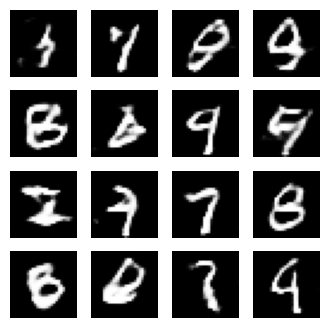
\includegraphics[width=.6\linewidth]{apendices/fig/9_IAA009_8.png}
\caption*{Fonte: O autor (2024).}
\end{figure}

%%%%%%%%%%%%%%%%%%%%%%%%%%%%%%%%%%%%%%%%%%%%%%%%%%%%%%%%%%%%%%%%%%%%%%%%%%%%%%%%%%%%%%%%%%%
\begin{adjustwidth}{1em}{}
\textbf{4 Tradutor de Textos (Transformer)}
\end{adjustwidth}


\begin{lstlisting}[language=Python, style=input]
# Instalação e importação
!pip uninstall -y tensorflow
!pip uninstall -y tf-keras
!pip install tf-keras==2.15.1
!pip install tensorflow==2.15.0 #--use-deprecated=legacy-resolver
!pip install tensorflow_datasets
!pip install -U tensorflow-text==2.15.0
pip install matplotlib

import collections
import logging
import os
import pathlib
import re
import string
import sys
import time

import numpy as np
import matplotlib.pyplot as plt

import tensorflow_datasets as tfds
import tensorflow_text as text
import tensorflow as tf

logging.getLogger('tensorflow').setLevel(logging.ERROR)  # suppress warnings

# Carregar a base de dados
examples, metadata = tfds.load('ted_hrlr_translate/pt_to_en', with_info=True, as_supervised=True)
train_examples, val_examples = examples['train'], examples['validation']

# Verificar o dataset
for pt_examples, en_examples in train_examples.batch(3).take(1):
  for pt in pt_examples.numpy():
    print(pt.decode('utf-8'))
  print()

  for en in en_examples.numpy():
    print(en.decode('utf-8'))
\end{lstlisting}

\begin{tcolorbox}[myoutputstyle]
e quando melhoramos a procura , tiramos a única vantagem da impressão , que é a serendipidade .\\
mas e se estes fatores fossem ativos ?\\
mas eles não tinham a curiosidade de me testar .\\
\\
and when you improve searchability , you actually take away the one advantage of print , which is serendipity .\\
but what if it were active ?\\
but they did n't test for curiosity .
\end{tcolorbox}


\begin{lstlisting}[language=Python, style=input]
# Tokenização e Destokenização do texto
model_name = "ted_hrlr_translate_pt_en_converter"

tf.keras.utils.get_file(f"{model_name}.zip", f"https://storage.googleapis.com/download.tensorflow.org/models/{model_name}.zip", cache_dir='.', cache_subdir='', extract=True)
# Tem 2 tokenizers: um pt outro em en tokenizers.en tokeniza e detokeniza
tokenizers = tf.saved_model.load(model_name)

# PIPELINE DE ENTRADA
# Codificar/tokenizar lotes de texto puro
def tokenize_pairs(pt, en):
  pt = tokenizers.pt.tokenize(pt)
  # Converte ragged (irregular, tam variável) para dense
  # Faz padding com zeros.
  pt = pt.to_tensor()

  en = tokenizers.en.tokenize(en)
  # ragged -> dense
  en = en.to_tensor()
  return pt, en

# Pipeline simpes: processa, embaralha, agrupa os dados, prefetch
# Datasets de entrada terminam com prefetch
BUFFER_SIZE = 20000
BATCH_SIZE = 64

def make_batches(ds):
  return (
    ds
    .cache()
    .shuffle(BUFFER_SIZE)
    .batch(BATCH_SIZE)
    .map(tokenize_pairs, num_parallel_calls=tf.data.AUTOTUNE)
    .prefetch(tf.data.AUTOTUNE)
  )

train_batches = make_batches(train_examples)
val_batches = make_batches(val_examples)

# CODIFICACAO POSICIONAL
def get_angles(pos, i, d_model):
  angle_rates = 1 / np.power(10000, (2 * (i//2)) / np.float32(d_model))
  return pos * angle_rates

def positional_encoding(position, d_model):
  angle_rads = get_angles(np.arange(position)[:, np.newaxis],np.arange(d_model)[np.newaxis, :],d_model)
  # sin em índices pares no array; 2i
  angle_rads[:, 0::2] = np.sin(angle_rads[:, 0::2])
  # cos em índices ímpares no array; 2i+1
  angle_rads[:, 1::2] = np.cos(angle_rads[:, 1::2])
  # newaxis, aumenta a dimensão [] -> [ [] ]

  pos_encoding = angle_rads[np.newaxis, ...]
  return tf.cast(pos_encoding, dtype=tf.float32)

# CODIFICACAO POSICIONAL
n, d = 2048, 512
pos_encoding = positional_encoding(n, d)
print(pos_encoding.shape)
pos_encoding = pos_encoding[0]

# Arrumar as dimensões
pos_encoding = tf.reshape(pos_encoding, (n, d//2, 2))
pos_encoding = tf.transpose(pos_encoding, (2, 1, 0))
pos_encoding = tf.reshape(pos_encoding, (d, n))

plt.pcolormesh(pos_encoding, cmap='RdBu')
plt.ylabel('Depth')
plt.xlabel('Position')
plt.colorbar()
plt.show()
\end{lstlisting}


\begin{figure}[H]
\centering
\caption{Colomesh - Transformer}
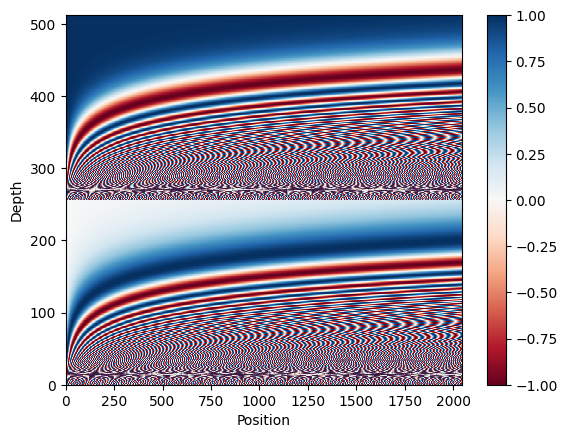
\includegraphics[width=.7\linewidth]{apendices/fig/9_IAA009_9.png}
\caption*{Fonte: O autor (2024).}
\end{figure}


\begin{lstlisting}[language=Python, style=input]
# Cria uma máscara de 0 e 1, 0 para quando há valor e 1 quando não há
def create_padding_mask(seq):
  seq = tf.cast(tf.math.equal(seq, 0), tf.float32)
  # add extra dimensions to add the padding
  # to the attention logits.
  return seq[:, tf.newaxis, tf.newaxis, :]  # (batch_size, 1, 1, seq_l)

# Máscara futura, usada no decoder
def create_look_ahead_mask(size):
  # zera o triângulo inferior
  mask = 1 - tf.linalg.band_part(tf.ones((size, size)), -1, 0)
  return mask # (seq_len, seq_len)

# Função de Atenção
def scaled_dot_product_attention(q, k, v, mask):
  # Q K^T
  matmul_qk = tf.matmul(q, k, transpose_b=True)  # (..., seq_len_q, seq_len_k)
  # converte matmul_qk para float32
  dk = tf.cast(tf.shape(k)[-1], tf.float32)

  # divide por sqrt(d_k)
  scaled_attention_logits = matmul_qk / tf.math.sqrt(dk)

  # Soma a máscara, e os valores faltantes serão um número próximo a -inf
  if mask is not None:
    scaled_attention_logits += (mask * -1e9)

  # softmax normaliza os dados, soman 1. // (..., seq_len_q, seq_len_k)
  attention_weights = tf.nn.softmax(scaled_attention_logits, axis=-1)
  output = tf.matmul(attention_weights, v)  # (..., seq_len_q, depth_v)
  return output, attention_weights

# Atenção Multi-cabeças
class MultiHeadAttention(tf.keras.layers.Layer):
  def __init__(self, d_model, num_heads):
    super(MultiHeadAttention, self).__init__()
    self.num_heads = num_heads
    self.d_model = d_model
    assert d_model % self.num_heads == 0
    self.depth = d_model // self.num_heads

    self.wq = tf.keras.layers.Dense(d_model)
    self.wk = tf.keras.layers.Dense(d_model)
    self.wv = tf.keras.layers.Dense(d_model)

    self.dense = tf.keras.layers.Dense(d_model)

  def split_heads(self, x, batch_size):
    #"Separa a última dimensão em (num_heads, depth).Transpõe o resultado para o shape (batch_size, num_heads, seq_len, depth)"
    x = tf.reshape(x, (batch_size, -1, self.num_heads, self.depth))
    return tf.transpose(x, perm=[0, 2, 1, 3])

  def call(self, v, k, q, mask):
    batch_size = tf.shape(q)[0]

    q = self.wq(q)  # (batch_size, seq_len, d_model)
    k = self.wk(k)  # (batch_size, seq_len, d_model)
    v = self.wv(v)  # (batch_size, seq_len, d_model)

    q = self.split_heads(q, batch_size)  # (batch_size, num_heads, seq_len_q, depth)
    k = self.split_heads(k, batch_size)  # (batch_size, num_heads, seq_len_k, depth)
    v = self.split_heads(v, batch_size)  # (batch_size, num_heads, seq_len_v, depth)

    # Calcula a atenção para cada cabeça (de forma matricial)
    # scaled_attention.shape == (batch_size, num_heads, seq_len_q, depth)
    # attention_weights.shape == (batch_size, num_heads, seq_len_q, seq_len_k)
    scaled_attention, attention_weights = scaled_dot_product_attention(q, k, v, mask)

    # Troca a dimensão 2 com 1, para acertar o num_heads# (batch_size, seq_len_q, num_heads, depth)
    scaled_attention = tf.transpose(scaled_attention, perm=[0, 2, 1, 3])
    # Concatena os valores em: (batch_size, seq_len_q, d_model)
    concat_attention = tf.reshape(scaled_attention, (batch_size, -1, self.d_model))
    output = self.dense(concat_attention)  # (batch_size, seq_len_q, d_model)
    return output, attention_weights

def point_wise_feed_forward_network(d_model, dff):
  return tf.keras.Sequential([
    tf.keras.layers.Dense(dff, activation='relu'),  # (batch_size, seq_len, dff)
    tf.keras.layers.Dense(d_model)  # (batch_size, seq_len, d_model)
  ])

class EncoderLayer(tf.keras.layers.Layer):
  def __init__(self, d_model, num_heads, dff, rate=0.1):
    super(EncoderLayer, self).__init__()
    self.mha = MultiHeadAttention(d_model, num_heads)
    self.ffn = point_wise_feed_forward_network(d_model, dff)

    self.layernorm1 = tf.keras.layers.LayerNormalization(epsilon=1e-6)
    self.layernorm2 = tf.keras.layers.LayerNormalization(epsilon=1e-6)

    self.dropout1 = tf.keras.layers.Dropout(rate)
    self.dropout2 = tf.keras.layers.Dropout(rate)

  def call(self, x, training, mask):
    attn_output, _ = self.mha(x, x, x, mask)
    attn_output = self.dropout1(attn_output, training=training)
    out1 = self.layernorm1(x + attn_output)
    ffn_output = self.ffn(out1)
    ffn_output = self.dropout2(ffn_output, training=training)
    out2 = self.layernorm2(out1 + ffn_output)

    return out2

class DecoderLayer(tf.keras.layers.Layer):
  def __init__(self, d_model, num_heads, dff, rate=0.1):
    super(DecoderLayer, self).__init__()

    self.mha1 = MultiHeadAttention(d_model, num_heads)
    self.mha2 = MultiHeadAttention(d_model, num_heads)
    self.ffn = point_wise_feed_forward_network(d_model, dff)

    self.layernorm1 = tf.keras.layers.LayerNormalization(epsilon=1e-6)
    self.layernorm2 = tf.keras.layers.LayerNormalization(epsilon=1e-6)
    self.layernorm3 = tf.keras.layers.LayerNormalization(epsilon=1e-6)

    self.dropout1 = tf.keras.layers.Dropout(rate)
    self.dropout2 = tf.keras.layers.Dropout(rate)
    self.dropout3 = tf.keras.layers.Dropout(rate)

  def call(self, x, enc_output, training, look_ahead_mask, padding_mask):
    # enc_output.shape == (batch_size, input_seq_len, d_model)
    # (batch_size, target_seq_len, d_model)
    attn1, attn_weights_block1 = self.mha1(x, x, x, look_ahead_mask)
    attn1 = self.dropout1(attn1, training=training)
    out1 = self.layernorm1(attn1 + x)

    # (batch_size, target_seq_len, d_model)
    attn2, attn_weights_block2 = self.mha2(enc_output, enc_output, out1, padding_mask)
    attn2 = self.dropout2(attn2, training=training)
    out2 = self.layernorm2(attn2 + out1)  # (batch_size, target_seq_len, d_model)

    ffn_output = self.ffn(out2)  # (batch_size, target_seq_len, d_model)
    ffn_output = self.dropout3(ffn_output, training=training)
    out3 = self.layernorm3(ffn_output + out2)  # (batch_size, target_seq_len, d_model)

    return out3, attn_weights_block1, attn_weights_block2

class Encoder(tf.keras.layers.Layer):
  def __init__(self, num_layers, d_model, num_heads, dff, input_vocab_size, maximum_position_encoding, rate=0.1):
    super(Encoder, self).__init__()
    self.d_model = d_model
    self.num_layers = num_layers
    self.embedding = tf.keras.layers.Embedding(input_vocab_size, d_model)
    self.pos_encoding = positional_encoding(maximum_position_encoding, self.d_model)
    self.enc_layers = [EncoderLayer(d_model, num_heads, dff, rate) for _ in range(num_layers)]
    self.dropout = tf.keras.layers.Dropout(rate)

  def call(self, x, training, mask):
    seq_len = tf.shape(x)[1]
    # adding embedding and position encoding.
    x = self.embedding(x)  # (batch_size, input_seq_len, d_model)
    x *= tf.math.sqrt(tf.cast(self.d_model, tf.float32))
    x += self.pos_encoding[:, :seq_len, :]
    x = self.dropout(x, training=training)
    for i in range(self.num_layers):
      x = self.enc_layers[i](x, training, mask)
    return x # (batch_size, input_seq_len, d_model)

class Decoder(tf.keras.layers.Layer):
  def __init__(self, num_layers, d_model, num_heads, dff, target_vocab_size,
    maximum_position_encoding, rate=0.1):
    super(Decoder, self).__init__()
    self.d_model = d_model
    self.num_layers = num_layers
    self.embedding = tf.keras.layers.Embedding(target_vocab_size, d_model)
    self.pos_encoding = positional_encoding(maximum_position_encoding, d_model)
    self.dec_layers = [DecoderLayer(d_model, num_heads, dff, rate) for _ in range(num_layers)]
    self.dropout = tf.keras.layers.Dropout(rate)

  def call(self, x, enc_output, training, look_ahead_mask, padding_mask):
    seq_len = tf.shape(x)[1]
    attention_weights = {}
    x = self.embedding(x)  # (batch_size, target_seq_len, d_model)
    x *= tf.math.sqrt(tf.cast(self.d_model, tf.float32))
    x += self.pos_encoding[:, :seq_len, :]
    x = self.dropout(x, training=training)
    for i in range(self.num_layers):
      x, block1, block2 = self.dec_layers[i](x, enc_output, training,look_ahead_mask, padding_mask)
      attention_weights[f'decoder_layer{i+1}_block1'] = block1
      attention_weights[f'decoder_layer{i+1}_block2'] = block2
    # x.shape == (batch_size, target_seq_len, d_model)
    return x, attention_weights

class Transformer(tf.keras.Model):
  def __init__(self, num_layers, d_model, num_heads, dff, input_vocab_size, target_vocab_size, pe_input, pe_target, rate=0.1):
    super().__init__()
    self.encoder = Encoder(num_layers, d_model, num_heads, dff, input_vocab_size, pe_input, rate)
    self.decoder = Decoder(num_layers, d_model, num_heads, dff, target_vocab_size, pe_target, rate)
    self.final_layer = tf.keras.layers.Dense(target_vocab_size)

  def call(self, inputs, training):
    # Keras models prefer if you pass all your inputs in the first argument
    inp, tar = inputs

    enc_padding_mask, look_ahead_mask, dec_padding_mask = self.create_masks(inp, tar)
    # (batch_size, inp_seq_len, d_model)
    enc_output = self.encoder(inp, training, enc_padding_mask)
    # dec_output.shape == (batch_size, tar_seq_len, d_model)
    dec_output, attention_weights = self.decoder(tar, enc_output, training, look_ahead_mask, dec_padding_mask)
    # (batch_size, tar_seq_len, target_vocab_size)
    final_output = self.final_layer(dec_output)

    return final_output, attention_weights

  def create_masks(self, inp, tar):
    # Encoder padding mask
    enc_padding_mask = create_padding_mask(inp)
    # Used in the 2nd attention block in the decoder.
    # This padding mask is used to mask the encoder outputs.
    dec_padding_mask = create_padding_mask(inp)
    # Used in the 1st attention block in the decoder.
    # It is used to pad and mask future tokens in the input received by
    # the decoder.
    look_ahead_mask = create_look_ahead_mask(tf.shape(tar)[1])
    dec_target_padding_mask = create_padding_mask(tar)
    look_ahead_mask = tf.maximum(dec_target_padding_mask, look_ahead_mask)
    return enc_padding_mask, look_ahead_mask, dec_padding_mask

# Hiperparâmetros
num_layers = 4
d_model = 128
dff = 512
num_heads = 8
dropout_rate = 0.1

class CustomSchedule(tf.keras.optimizers.schedules.LearningRateSchedule):
  def __init__(self, d_model, warmup_steps=4000):
    super(CustomSchedule, self).__init__()
    self.d_model = d_model
    self.d_model = tf.cast(self.d_model, tf.float32)
    self.warmup_steps = warmup_steps

  def __call__(self, step):
    step = tf.cast(step, tf.float32) # Adicionado para evitar ERRO
    arg1 = tf.math.rsqrt(step)
    arg2 = step * (self.warmup_steps ** -1.5)
    return tf.math.rsqrt(self.d_model) * tf.math.minimum(arg1, arg2)

learning_rate = CustomSchedule(d_model)
optimizer = tf.keras.optimizers.Adam(learning_rate, beta_1=0.9, beta_2=0.98, epsilon=1e-9)

loss_object = tf.keras.losses.SparseCategoricalCrossentropy(from_logits=True, reduction='none')

def loss_function(real, pred):
  mask = tf.math.logical_not(tf.math.equal(real, 0))
  loss_ = loss_object(real, pred)
  mask = tf.cast(mask, dtype=loss_.dtype)
  loss_ *= mask
  return tf.reduce_sum(loss_)/tf.reduce_sum(mask)

def accuracy_function(real, pred):
  accuracies = tf.equal(real, tf.argmax(pred, axis=2))
  mask = tf.math.logical_not(tf.math.equal(real, 0))
  accuracies = tf.math.logical_and(mask, accuracies)
  accuracies = tf.cast(accuracies, dtype=tf.float32)
  mask = tf.cast(mask, dtype=tf.float32)
  return tf.reduce_sum(accuracies)/tf.reduce_sum(mask)

train_loss = tf.keras.metrics.Mean(name='train_loss')
train_accuracy = tf.keras.metrics.Mean(name='train_accuracy')

transformer = Transformer(
  num_layers=num_layers,
  d_model=d_model,
  num_heads=num_heads,
  dff=dff,
  input_vocab_size=tokenizers.pt.get_vocab_size().numpy(),
  target_vocab_size=tokenizers.en.get_vocab_size().numpy(),
  pe_input=1000,
  pe_target=1000,
  rate=dropout_rate)

# Checkpoint
checkpoint_path = "./checkpoints/train"

ckpt = tf.train.Checkpoint(transformer=transformer, optimizer=optimizer)

ckpt_manager = tf.train.CheckpointManager(ckpt, checkpoint_path, max_to_keep=5)

# if a checkpoint exists, restore the latest checkpoint.
if ckpt_manager.latest_checkpoint:
  ckpt.restore(ckpt_manager.latest_checkpoint)
  print('Latest checkpoint restored!!')

EPOCHS = 20

train_step_signature = [
  tf.TensorSpec(shape=(None, None), dtype=tf.int64),
  tf.TensorSpec(shape=(None, None), dtype=tf.int64),
]
@tf.function(input_signature=train_step_signature)
def train_step(inp, tar):
  tar_inp = tar[:, :-1]
  tar_real = tar[:, 1:]
  with tf.GradientTape() as tape:
    predictions, _ = transformer([inp, tar_inp], training = True)
    loss = loss_function(tar_real, predictions)

  gradients = tape.gradient(loss, transformer.trainable_variables)
  optimizer.apply_gradients(zip(gradients, transformer.trainable_variables))

  train_loss(loss)
  train_accuracy(accuracy_function(tar_real, predictions))

for epoch in range(EPOCHS):
  start = time.time()
  train_loss.reset_state()
  train_accuracy.reset_state()

  # inp -> portuguese, tar -> english
  for (batch, (inp, tar)) in enumerate(train_batches):
    train_step(inp, tar)
    if batch % 50 == 0:
      print(f'Epoch {epoch + 1} Batch {batch} Loss {train_loss.result():.4f} Accuracy{train_accuracy.result():.4f}')

  if (epoch + 1) % 5 == 0:
    ckpt_save_path = ckpt_manager.save()
    print(f'Saving checkpoint for epoch {epoch+1} at {ckpt_save_path}')

  print(f'Epoch {epoch + 1} Loss {train_loss.result():.4f} Accuracy{train_accuracy.result():.4f}')
  print(f'Time taken for 1 epoch: {time.time() - start:.2f} secs\n')
\end{lstlisting}

\begin{tcolorbox}[myoutputstyle]
...\\
Epoch 20 Batch 0 Loss 1.4398 Accuracy0.6776\\
Epoch 20 Batch 50 Loss 1.4214 Accuracy0.6838\\
Epoch 20 Batch 100 Loss 1.4334 Accuracy0.6820\\
Epoch 20 Batch 150 Loss 1.4287 Accuracy0.6833\\
Epoch 20 Batch 200 Loss 1.4364 Accuracy0.6820\\
Epoch 20 Batch 250 Loss 1.4398 Accuracy0.6815\\
Epoch 20 Batch 300 Loss 1.4402 Accuracy0.6813\\
Epoch 20 Batch 350 Loss 1.4458 Accuracy0.6804\\
Epoch 20 Batch 400 Loss 1.4458 Accuracy0.6805\\
Epoch 20 Batch 450 Loss 1.4450 Accuracy0.6804\\
Epoch 20 Batch 500 Loss 1.4463 Accuracy0.6801\\
Epoch 20 Batch 550 Loss 1.4490 Accuracy0.6795\\
Epoch 20 Batch 600 Loss 1.4511 Accuracy0.6793\\
Epoch 20 Batch 650 Loss 1.4533 Accuracy0.6788\\
Epoch 20 Batch 700 Loss 1.4567 Accuracy0.6782\\
Epoch 20 Batch 750 Loss 1.4590 Accuracy0.6778\\
Epoch 20 Batch 800 Loss 1.4610 Accuracy0.6775\\
Saving checkpoint for epoch 20 at ./checkpoints/train/ckpt-4\\
Epoch 20 Loss 1.4617 Accuracy0.6774\\
Time taken for 1 epoch: 95.57 secs
\end{tcolorbox}


\begin{lstlisting}[language=Python, style=input]
class Translator(tf.Module):
  def __init__(self, tokenizers, transformer):
    self.tokenizers = tokenizers
    self.transformer = transformer
  def __call__(self, sentence, max_length=20):
    # input sentence is portuguese, hence adding the start and end token
    assert isinstance(sentence, tf.Tensor)
    if len(sentence.shape) == 0:
      sentence = sentence[tf.newaxis]
    sentence = self.tokenizers.pt.tokenize(sentence).to_tensor()
    encoder_input = sentence
    # as the target is english, the first token to the transformer should be the
    # english start token.
    start_end = self.tokenizers.en.tokenize([''])[0]
    start = start_end[0][tf.newaxis]
    end = start_end[1][tf.newaxis]
    output_array = tf.TensorArray(dtype=tf.int64, size=0, dynamic_size=True)
    output_array = output_array.write(0, start)
    for i in tf.range(max_length):
      output = tf.transpose(output_array.stack())
      predictions, _ = self.transformer([encoder_input, output], training=False)
      predictions = predictions[:, -1:, :]  # (batch_size, 1, vocab_size)
      predicted_id = tf.argmax(predictions, axis=-1)
      output_array = output_array.write(i+1, predicted_id[0])
      if predicted_id == end:
        break

    output = tf.transpose(output_array.stack())
    # output.shape (1, tokens)
    text = tokenizers.en.detokenize(output)[0]
    tokens = tokenizers.en.lookup(output)[0]
    _, attention_weights = self.transformer([encoder_input, output[:,:-1]], training=False)
    return text, tokens, attention_weights

translator = Translator(tokenizers, transformer)

sentence = "Eu li sobre triceratops na enciclopédia."

translated_text, translated_tokens, attention_weights = translator(tf.constant(sentence))

print(f'{"Prediction":15s}: {translated_text}')
\end{lstlisting}

\begin{tcolorbox}[myoutputstyle]
Prediction     : b'i read about tribucis in egypt .'
\end{tcolorbox}